\chapter{Product development}
This chapter describes the technical side of this project. The technologies used, the network peripherals and the architecture of the iCare system are discussed here.

\section{Basic architecture}
In order to give the user as much freedom as possible and to save him the installation and administration of unnecessary software and unnecessary software components, this project is implemented as a web server. This means that the system can be accessed by every employee under their user ID and password via the Internet using a web browser. The user interface elements are designed to be comfortably operated from a desktop PC as well as from mobile devices such as tablets and smartphones. This makes the iCare system platform independent and supports an easy and elegant user experience. The intention is to make it as easy as possible for the user to use the iCare system by using technologies that every user can use intuitively.

\subsection{iCare Network}
The server uses both wireless connections and the Ethernet connection within the care home to communicate with all connected devices as well as the backup system. As already described in chapter \ref{basic-concept}, each room within the care home has a network HUB, which is connected to the central server via Ethernet. This network HUB communicates either via an Ethernet connection or via a wireless connection with the devices installed in the room. Figure \ref{icare-network} shows the network peripherals of the iCare system:
\begin{figure}[H]
	\centering
	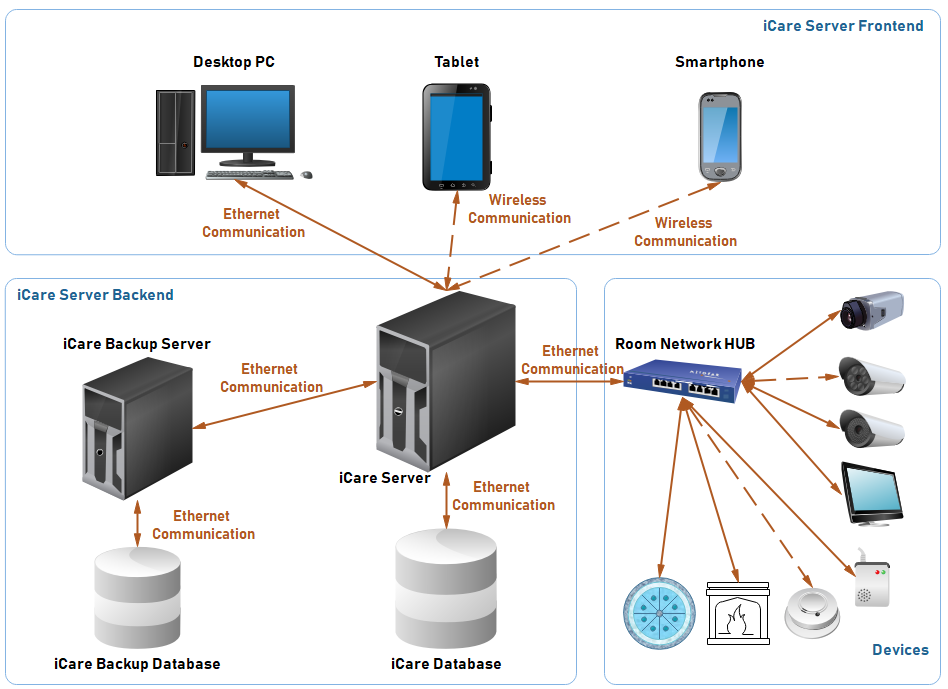
\includegraphics[width =1.0\textwidth]{images/iCare-Network.PNG}
	\caption{iCare Network}
	\label{icare-network}
\end{figure}
The solid lines represent communication via Ethernet cabling, while the dashed lines indicate a wireless connection. The devices connected to the network HUB are already listed in the overview in chapter \ref{basic-concept} for each room and are not considered here. A detailed examination of the individual devices can be found in the hardware calculation in Chapter \ref{market-analysis}.

\subsection{iCare Communication}
The data collected by the devices in the individual rooms is forwarded to the central server via the network HUB. The server analyzes this data, persists it in the database, forwards it to the backup system, and prepares it for display in the frontend of the iCare system. The processed data will also be forwarded to the infoboard for presentation via the network hub of the community room. It is also possible to access and control the devices for central heating and water consumption via the network HUB. For the frontend, it is also possible to send user inputs and user requests to the central server at any time, which then processes them and returns the corresponding results to the frontend. These data and control flows are shown in figure \ref{icare-dataflow}.
\begin{figure}[H]
	\centering
	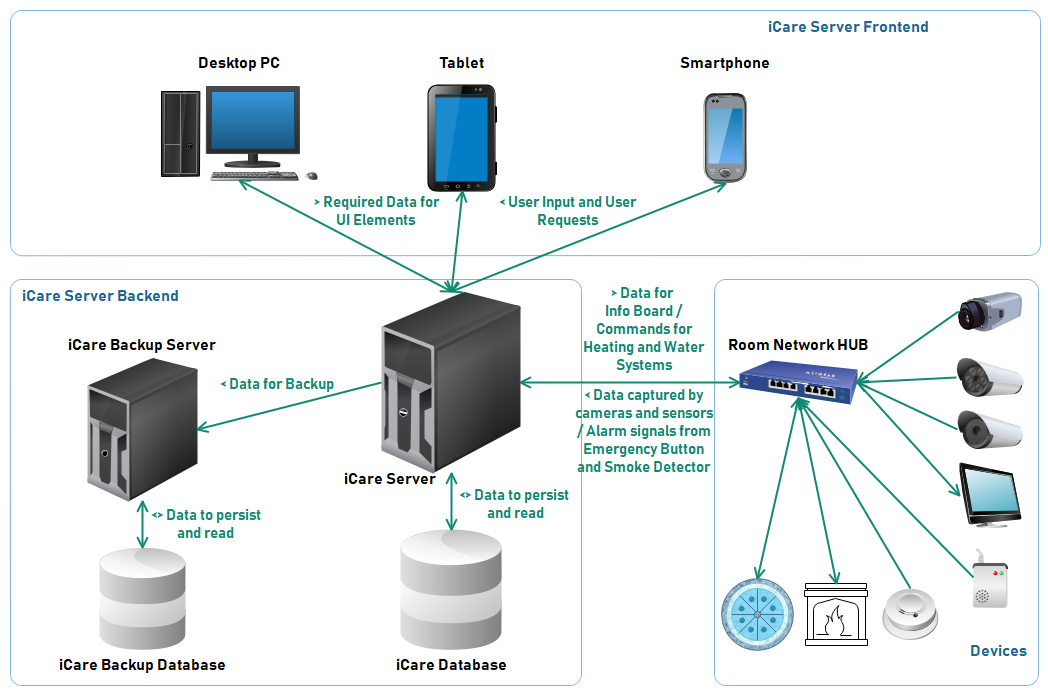
\includegraphics[width =1.05\textwidth]{images/iCare-Dataflow.PNG}
	\caption{iCare control- and data- flows}
	\label{icare-dataflow}
\end{figure}

A more detailed description of the individual subsystems will be given in the next chapters. It focuses on how the communication between the frontend and the backend of the iCare server is implemented, which data model is used, and which features the server offers the user.
